\section{Traitement de Langage Naturel (TLN)}
\subsection{Introduction}
Le Traitement de Langage Naturel (Natural Langage Processing) est une approche pour analyse des textes qui est basé sur les théories et la téchnologies. C'est un domaine très répandu actuellement dans la recherche et developpement \citep{natural-language-processing}. La NLP est utilisé dans la recherche d'information, traduction des textes, traduction des voix, système de question reponse ainsi que diverses domaines.

\begin{definition}[NLP]
    Natural Language Processing (NLP) est un discipline qui combine la linguistique, l'informatique et l'intelligence artificielle pour analyser et etudier les intéractions entre uns système informatique et une langage naturel humain. La Recherche d'Information est parmi l'une de tâche du NLP \citep{art-nlp}.
\end{definition}

\begin{definition}[NLP]
    Selon \citeauthor{natural-language-processing}, un NLP est un ensemble des téchniques informatiques théoriques motivés pour analyser et represeter naturellement des textes (un langage quelconque) en passant par un ou plusieurs niveaux d'analyse linguistique dans le but de parvenir a traiter le langage humain dans un étendu de tâches ou applications \citep{natural-language-processing}.
\end{definition}

L'analyse de langage, porte a connaitre la structure de langage tel que les mots, les significations, combinaison des mots, ainsi que la contribution des mots au sense de la phrase. Et aussi d'analyser le fonctionnemet du monde et le raisonnement de l'humanité dans le monde \citep{automatic-nlp}.

Le domaine de TLN a quelques divisions tel que:
\begin{itemize}
    \item \textbf{NLP}: production de representation significatif. Equivalent du rôle de lecteur et ecouteur.
    \item \textbf{NLG}: production de langage a partir d'une representation. Equivalent du role d'auteur et interlocuteur.
    \item \textbf{Language Understanding}: Termine avec un langage orale.
    \item \textbf{Speech Understanding}: Demarre avec un langage orale. Permet de savoir comment un langage orale va se traduire en texte.
\end{itemize}

Le domaine NL par rapport a l'intelligence artificielle est illustré dans la Figure~\ref{fig:nlp-ref-ai}.

\begin{figure}[htbp]
    \begin{center}
        \fbox{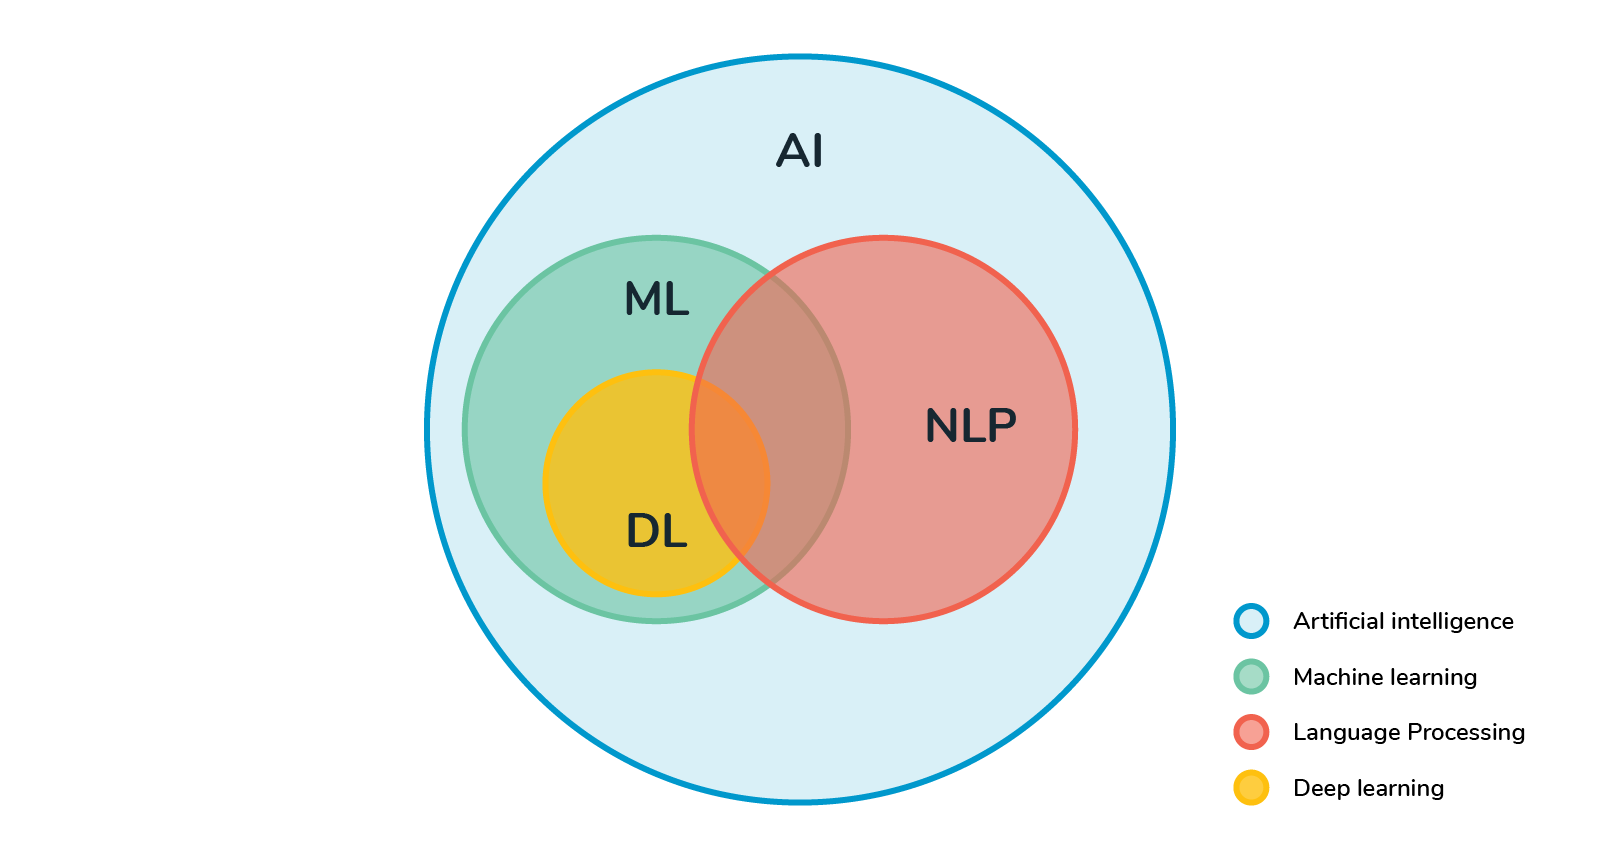
\includegraphics[width=13cm, angle=0]{Figures/NLP/nlp-ref-ai.png}}
    \end{center}
    \caption{Position du TLN par rapport a l'IA \citep{devopedia-nlp}}
    \label{fig:nlp-ref-ai}
\end{figure}

Certains notion qu'on abordera ici sont déja presenté dans la section (Processus de recherche d'information), donc certains notions ne seront pas détaillés.

\subsection{Un peu d'histoire}
Cette briève historique est tiré de l'ouvrage de \citeauthor{natural-language-processing} \citep{natural-language-processing}. La recherche en Traitement de Langage Natures trouve ses origines dans les années 1940. Le MT (Machine Translation) est la prémière application en NLP qui est une application d'ordinateur. En 1946, Weaver et Booth demarre l'une de projet recent de MT, encore sur la traduction basé sur l'expertise de voler le code d'énemie durant la deuxième guerre mondiale. Ce projet a suggerré l'utilisation de la cryptographie et de la théorie de l'information pour le traduction de langage. Puis la recherche sont devenu varié dans les institutions en Etats-Unis d'Amérique (USA).

En 1957, Chomsky a publié Syntactic Structure, qui introduit l'idée de grammaire génerative pour remedier aux problèmes rencontré dans les années anérieurs tel que l'ambiguité syntaxique, \dots Une autre domaine de NLP commence aussi a emerger, qui est la reconnaissance vocale.

La communauté de Traitement de langage et la communauté vocale (Speech community) était divisé alors en deux camps: d'une part la communauté de traitement de langage dominé par la théorie perspective de grammaire generative et hostile en methode statistique; et d'autre part la communauté vocal (SC) dominé par la théorie statistique de l'information et hostile en théorie linguistique.

En 1950, l'homme pense que la meilleur qualité totalement automatique peut produire des resultats indiscernable de la translation huamine, et qu'un tel système peut être opérationnel dans quelques années.

Enfin, la NLP a connu beaucoup d'évolution ainsi des nombreuses lacunes. A partir des années 1980, la NLP a evolué beaucoup plus vite par la dispositions des ressources computationel ainsi que des ordinateurs performants.

\subsection{Les niveaux de langage}
Un langage comporte géneralement cinq niveaux ou étape de traitement \citep*{automatic-nlp, handbook-nlp} et qui est illustré dans la Figure~\ref{fig:nlp-stage}:
\begin{itemize}
    \item \textbf{Phonétique et phonologie}: la liaison des mots et des phrases au son qui les réalisent a l'oral. Cette niveau n'est past utile dans le traitement de langage textuelle.
    \item \textbf{Morphologie}: la façon dont les mots sont construits, et de connaitre leurs rôles dans la phrase.
    \item \textbf{Syntaxe}: la façon dont les mots se combinent pour former des \textit{syntagmes}, puis des proposition et enfin des phrases correctes. Un \textbf{syntagmes} est un unité syntaxique intermédiaire entre le mot et la prase, et comprenant un seul noyau et souvent des compléments.
    \item \textbf{Sémantique}: la façon dont les mots font du sens lorsqu'ils sont insérés dans une phrase indépendamment du contexte.
    \item \textbf{Pragmatique}: la façon d'interpreter les phrases selon leur contexte d'énonciation comme l'interlocuteur, phrase précedente, connaissance commune du monde, \dots
\end{itemize}

\begin{figure}[htbp]
    \begin{center}
        \fbox{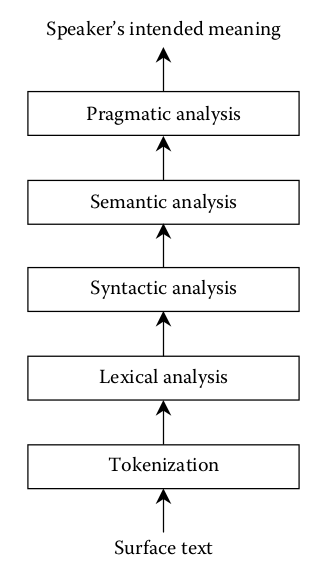
\includegraphics[width=8cm, angle=0]{Figures/NLP/nlp-stage.png}}
    \end{center}
    \caption{Etape d'analyse de texte dans NLP \citep{handbook-nlp}}
    \label{fig:nlp-stage}
\end{figure}

\subsection{Phonologie}
La phonologie interprète le langage parlé (son de parole) dans un mot \citep{natural-language-processing}. Il y a trois règles tel que:
\begin{itemize}
    \item \textbf{Règle phonétique}: pour les sons dans les mots.
    \item \textbf{Règle phonémique}: pour les variations de prononciation quand les mots son prononcé ensemble.
    \item \textbf{Règle prosodique}: pour la variation d'un stresse et d'intonation dans un phrase.
\end{itemize}

\subsection{Morphologie}
La morphologie est l'étude de la forme des mots tel que leur \textit{fléxion}: indication de cas, genre, nombre, mode et temps; leur \textit{derivation}: préfixes, suffixes et infixes; leur \textit{composition}: mots composés. C'est aussi une analyse morphosyntaxique, qui analyse des règles de combinaison des morphèmes selon la configuration syntaxique de l'énnoncé. La morphologie consiste a segmenter des textes en unités élémentaire qu'on appelle \textit{tokenisation} et à determiner les différentes caractéristiques de ces unités \citep{automatic-nlp,natural-language-processing}.

Un humain est capable de faire ce traitement pour comprendre le sens, vu que chaque sens des morphèmes ne change pas dans tous les mots, et idem pour un système NLP qui consiste a reconnaitre le sens porté par chaque morphème pour representer le sens \citep{natural-language-processing}.

\begin{definition}[Lemme]
    On appelle \textit{lemme} la racine d’un mot, sans ses marques d’accord, de conjugaison, de cas. L'entrée d'un dictionnaire est généralement un lemme. Le lemme est necessaire dans toute analyse sémantique. \citep{automatic-nlp}
\end{definition}

\begin{definition}[Flexion]
    Les \textit{flexions} sont les modifications opérées sur le lemme pour distinguer les formes de conjugaison (personne, temps, mode, voix – flexion verbale) ou le genre, le nombre et le cas (flexion nominale).L’opération qui consiste à retrouver ces informations est la \textit{lemmatisation}, ou souvent appellé \textit{racinisation (stemming)} \citep{automatic-nlp}.
\end{definition}

\begin{definition}[Morphème]
    On appelle \textit{morphème} le plus pétit unité ou unité minimale de sens \citep{natural-language-processing}. Par exemple, le mot pretraitement est composé de trois morphèmes tel que le prefix \textbf{pre}, la racine \textbf{traite} et la suffixe \textbf{ment}.
\end{definition}

Cette étape est une parite essentiel du NLP, qui est necessaire pour definir les caractères, mots et phrases dans un document. Cette rélève un défi tel que la résolution des ambiguités dans le langage naturel ainsi que de convertir des fichiers textes dans un séquence de texte bien défini eavec un sens. Cette étape peut être divisé en deux parties: \textit{Triage de document (Document Triage)} et \textit{Ségmentation de texte (Text Segmentation)} \citep{handbook-nlp}.

\subsubsection{Triage de document}
Le triage de document c'est l'action de convertir un ensemble des fichiers en documents textuelles bien définie. Il se decompose en trois étapes tel que:
\begin{enumerate}
    \item \textbf{Identification d'encodage de caractère (Character Encoding Identificator)}: permet d'identifier l'encodage de caractère utilisé dans le fichier a convertir, par exemple si le fichier utilise l'encodage UTF-8 ou ISO ou autres.
    \item \textbf{Identification de langage (Language Identification)}: permet de determiner dans quelle langue le fichier est écrit (Français, Anglais, etc.).
    \item \textbf{Sectionnement de texte (Text Sectionning)}: permet d'identifier le conténu textuel du fichier pour pouvoir le convertir een document textuel bien défini.
\end{enumerate}

\subsubsection{Segmentation de texte}
La segmentation de texte est un étape cruciale et complexe dans la Traitement de Langage Naturel. Il consiste a convertir un document textuel bien déifnie en composant des mots et des phrases \citep{handbook-nlp}. C'est aussi la transformation d'un alignement d'un caractère en une unité élementaire souvent des mots et phrase \citep{automatic-nlp}. Généralement, il y a trois étapes tel que la \textit{ségmentation de mot (Word segmentation)}, la \textit{normalisation de texte (Text Normalization)} et la \textit{ségmentation de phrase (Sentnce Segmentation)}.

Pour la segmentation de texte, il faut éfinir une liste de caractères délimiteur pour pouvoir segmenter le texte (espace, ponctuation, apostrophe). Pour les langages dont l'espace n'est pas un délimiteur comme la langue chinoise par exemple, cette segmentation est plus complexe \citep{handbook-nlp}. Et même avec la langue qui a comme délimiteur les trois cités ci-dessus, il est encore compliqué de separé les mots, car l'apostrophe peut être utilisé dans un seul mot comme \textit{aujourd'hui}, aussi un unité élémentaire peut conténir des éspaces comme \textit{pomme de terre} \citep{automatic-nlp}.

En pratique le système de segmentation du texte utilise une liste de sépatateurs par defaut, a laquelle ils ajoutent des connaissances lexicales et morphosyntaxiques pour traiter les cas ambigus. Chaque lange possède ses propres connqissances léxicales.

\subsubsubsection*{Segmentation de mot}
La segmentation de mot c'est l'action couper un sequence des caractères en texte par la localisation de delimiteur de mot (Word boundaries) pour pouvoir être utilisé dans la traitement linguistique. Un délimiteur permet de définir le point où un mot est terminé et qu'un autre commence. Les mots obténues sont appelées des \textit{tokens}, et la façon d'obtenir ces tokens est la \textit{tokenisation ou tokenization en anglais}. \citep{handbook-nlp}

Pour les langages delimité par un espace (space-delimited), souvent des langages européennes, les mots sont séparés par des espaces. Tandis que pour des langages qui ne sont pas delimités par un espace comme le Chinois et le Thai, il n'y a pas d'indication sur le delimiteur \citep{handbook-nlp}. Dans le cadre de ce devoir, on travaillera sur des langages qui a comme délimiteur espace.

Dans un langage délimité par un espace, les ponctuations sont souvent traité comme des tokens separés, mais qui varie d'un langage a un autre. Masi souvent pose de problèmes comme des abbréviation, les quotes et les appostrophes. \citep{handbook-nlp}

\subsubsubsection*{Normalisation de texte}
La normalisation de texte permet de fusionner les différentes formes de token en une forme canonique normalisé par exemple Mr et Monsieur. Cette normalisation permet aussi de normaliser des dates, des heures, des formats monétaires et d'autre informations numériques. Par exemple, les trois tokens écrit \$300 peut être prononcé comme \og{trois cent dollars} \fg{} et la normalisation de texte peut convertir le token original en token desiré. \citep{handbook-nlp}

\subsubsubsection*{Segmentation de phrase}
C'est de determiner comment le texte doit être divisé en phrase pour un traitement plus avancé. En identiiant les délimiteurs de phrase (souvent un point pour la langue delimité par un espace). Souvent la segmentation de phrase est referencé comme \textit{detection de dilimiteur de phrase} ou \textit{desambiguition de délimiteur de phrase} ou encore \textit{reconnaissance de délimiteur de phrase} \citep{handbook-nlp}.

\subsubsection{Catégories grammaticales}
Les catégories grammaticales est une information morphosyntaxique importante. Ces catégories sont souvent des noms, verbe, adjectif, mais qui varie selon le système. Par exemple \textit{Penn Treebank} contient 45 catégories. Sur la Figure~\ref{fig:categorie-grammaticale} un exemple de catégorie grammaticale pour la phrase \textit{\og Qui veut noyer son chien l’accuse de la rage \fg{}}, et qui illustre aussi la problème d'ambiguité pour cette phrase. En général 25\% du lexique est de forme ambigus pour la langue française. Et un exemple de description morphosyntaxique illustré dans la Figure~\ref{fig:exemple-desc-morphosyntaxique}.

\begin{figure}[htbp]
    \begin{center}
        \fbox{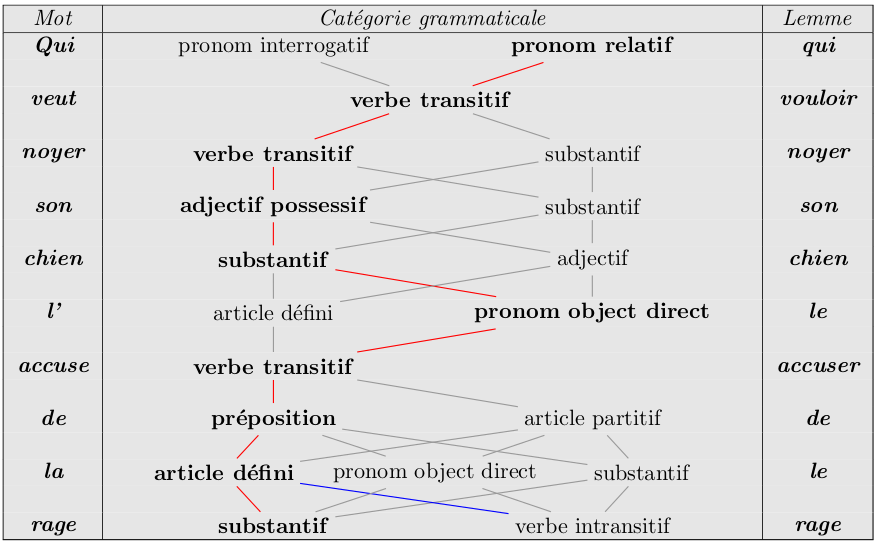
\includegraphics[width=15cm, angle=0]{Figures/NLP/classe-grammatical.png}}
    \end{center}
    \caption{Catégorie grammaticale \citep{handbook-nlp}}
    \label{fig:categorie-grammaticale}
\end{figure}

\begin{figure}[htbp]
    \begin{center}
        \fbox{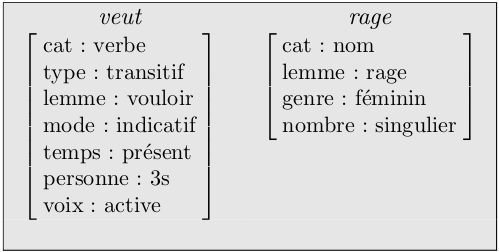
\includegraphics[width=10cm, angle=0]{Figures/NLP/description-morphosyntaxique.png}}
    \end{center}
    \caption{Description morphosyntaxique \citep{handbook-nlp}}
    \label{fig:exemple-desc-morphosyntaxique}
\end{figure}

\subsection{Analyse lexicale}
Un humain ou un Système NLP interptète le sens de chaque mot individuellement. L'analyse lexicale permet alors de determiner le sens de chaque mot individuellement. Le but est de contribuer au comprehension de niveau de mot par une affectation de tag \textit{part-of-speech} pour chaque mot. Un mot qui a un sens possible peut être remplacé par un representation semantique de ce sens \citep{natural-language-processing}.

Un analyse lexicale utilise un lexicon, qui est determiné et choisi par le système NLP. Un lexicon peut être \textbf{simple} c'est à dire des mots et ses \textit{pos} ou peut être \textbf{complexe} et contient l'information de classe sémantique des mots \citep{natural-language-processing}.

\subsection{Syntaxe}
La syntaxe décrit comment les lemmes ou fléxions sont ordonnées pour créer des constituants, composant aux-mêmes des phrases. Souvent, l'analyse syntaxique est representé de façon hierarchique. Dans l'analyse syntaxique, on travaille avec les mots, les phrases, ainsi que l'étape de la formation du mots a la phrase \citep{automatic-nlp}. L'analyse syntaxique est une analyse complexe avec différentes niveaux, les détails ne seront pas traité dans ce dévoir, mais présent dans \citetitle[section 3]{automatic-nlp} \citep{automatic-nlp}.

L'analyse syntaxique selon \citeauthor{natural-language-processing}, se focalise sur l'analyse des mots dans une phrase, pour decouvrir la structure grammaricale de la phrase, qui necessite l'utilisation de la grammaire et un parseur. Dans l'analye syntaxique, l'ordre et le depenance des mots contribue au sens: par exemple, la phrase \textit{\og Le chat attaque le chien \fg{}} et la phrase \textit{\og Le chien attaque le chat \fg{}} ont un sens différent car ses termes de sytaxe est différent, pourtant ils sont composé des mêmes mots \citep{natural-language-processing}.

\subsubsection{Analyse syperficielle}
Le but de l'analyse superficielle ou partielle \citep{automatic-nlp}, est de reconnaitre les syntagmes simples, non récursif d'un énoncé sans lier les uns aux autres; d'obtenir des résultats moins riches mais plus sûr et plus rapide. Cette approche s'oppose a l'analyse profonde ou complète qui cherche a regrouper chaque phrase dans une unique representation.

\textbf{Cass} est un exemple de d'analyseur partielle efficace, qui consiste en une cascade d'automates à états finis.

\subsubsection{Analyse en dépendance}
L’analyse syntaxique en dépendance diffère surtout de l’analyse en constituants (comme les règles hors-contexte) par le mode de représentation. Les deux approches n’ont pas de différence au niveau de leur couverture ou de leur expressivité (A reformuler). L'idée est de relier les mots et non les constituants \citep{automatic-nlp}.

Un exemple de grammaire de dépendance est la \emph{Link Grammar} qui définit la lexique et les contraintes d'attachement, comme illustré dans la Figure~\ref{fig:link-grammar} et la Figure~\ref{fig:link-grammar-syntax}

\begin{figure}[htbp]
    \begin{center}
        \fbox{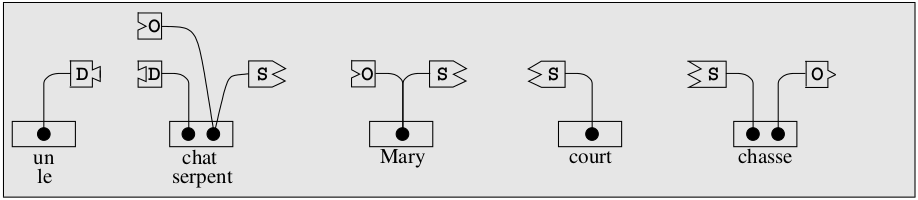
\includegraphics[width=13cm, angle=0]{Figures/NLP/lexic-link-grammar.png}}
    \end{center}
    \caption{Exemple de définition de la lexique \emph{Link Grammar} \citep{automatic-nlp}}
    \label{fig:link-grammar}
\end{figure}

\begin{figure}[htbp]
    \begin{center}
        \fbox{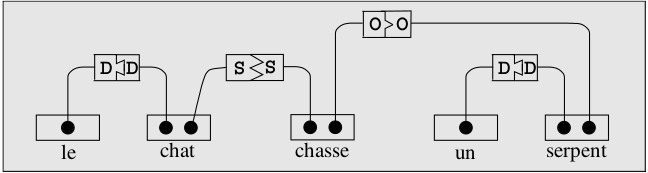
\includegraphics[width=13cm, angle=0]{Figures/NLP/syntax-link-grammar.png}}
    \end{center}
    \caption{Exemple d'analyse syntaxique avec \emph{Link Grammar} \citep{automatic-nlp}}
    \label{fig:link-grammar-syntax}
\end{figure}

\subsection{Sémantique}
Un approche sémantique peut être utilisé pour reduire les ambiguités syntaxiques, a mieux cibler des contextes (en RI par exemple), mais son but finale est de représenter formellement l’information véhiculée par un énoncé et éventuellement d’en inférer de nouvelles connaissances ou une réponse à la question posée dans le cas où l'énoncé est une question \citep{automatic-nlp}. Il a pour but d'associer a un sequence de mots une répresentation interne de son sens, tout en prenant compte l'utilisation futures des resultats obtenues.

Selon beaucoup des personnes, c'est dans le niveau sémantique qu'on determine la signification, pourtant tous les niveaux contribuent au signification. La sémantique determine alors la signification possible d'une phrase en se concentrant sur l'interaction parmi les significations de niveau des mots dans une phrase, avec la possibilité de desambiguition sémantique des mots aux multiple sens. Par exemple si on prend le mot \textbf{pile}, ca peut être un pile pour alimenter un appareil electronique, ou ca peut être un structure dans un langage de programmation informatique.

Selon \citeauthor{automatic-nlp}, il y a quatres méthodes:
\begin{itemize}
    \item \textbf{L'analyse profonde}: permet d'obtenir une representation complète de l'enoncé
    \item \textbf{Interpretation sémantique grammaticales}: qui s'appuie sur une analyse syntaxique totale
    \item \textbf{Grammaires sémantiques}: qui modelisent les données spécifiques
    \item \textbf{Patrons sémantique}: qui detectent les informations prédefinies dans un texte
\end{itemize}

On distingue deux types de sémantique tel que la \textit{sémantique grammaticale} qui se charge a construire un sens de l'énoncé globale, et la \textit{sémantique lexical} qui étudie la participation des mots a ce sens et tous les ambiguités qu'ils provoquent.

\citeauthor{amelioration-ri-approche-semantique,approche-semantique} \citep{amelioration-ri-approche-semantique,approche-semantique} ont chacun developpé un moteur de recherche basé sur cette notion de sémantique pour ameliorer la qualité de recherche, et analyser les ambiguités dans un terme de recherche des utilisateurs.

\subsubsection*{Quelques rélations importantes entre les mots}
Il y a des relations importantes entre les mots \citep{automatic-nlp} qui est necessaire en analyse sémantique tel que:
\begin{itemize}
    \item \textbf{Polysémie et l'homonymie}: propriété de certains formes graphiques (signifiants) de renvoyer à plusieurs sens (signifié). Par exemple, le mot \textit{bureau}.
    \item \textbf{Synonmie}: lien entre deux mots ayant la même sens.
    \item \textbf{Hyponymie}: relation d'inclusion entre deux mots dont l'un (hyponymie) est plus spécifique que l'autre (hyperonyme). Par exemple le mot \textit{gorille} est un hyponimie du mot \textit{quadrimane}, le mot \textit{fleur} est un hyperonymie du mot \textit{tulipe}.
    \item \textbf{Méronymie et holonymie}: relation de partie a tout. Par exemple, une serrure est une partie d'une cage (meronymie), un batiment contient une pièce (holonymie).
\end{itemize}

Ces relations existant entre les mots sont repertoriés dans des base informatiques dont le plus utilisés est \textbf{WORDNet}.

\subsection{Pragmatique}
\citeauthor{natural-language-processing} cite un niveau supplémentaire entre la sémantique et la pragmatique, c'est le \textbf{discours} qui travaille sur un texte plus longue qu'une phrase et interprète le sens en connectant tous les phrases. Il y a deux types de traitement de discours tel que: l'\textit{Anaphora} et le \textit{Discours/text structure recognition}.

Tandis que l'analyse pragmatique sert dans un sitiation bien spécifique, utilise de contexte qui dépasse le contenu de comprehension de texte \citep{natural-language-processing}. En d'autres termes, regroupe un grand nombre de domaine qui englobent tous les problèmes qui ne pouvant être traités avec la syntaxe et la sémantique \citep{automatic-nlp}. Cette analyse necessite l'utilisation des connaissances extra-linguistiques sur le contexte et du discours. Pour cette raison que les application pratiques sont rares, pourtant il y a quelques uns \citep{automatic-nlp} comme la \textit{diéctique}, l'\textit{implicateurs conversationnelle} et la \textit{presupposition}.

\subsection{Approche du TLN}
Il y a généralement trois approche dans la Traitement de Langage Naturel, tel que l'\textit{approche symbolique}, l'\textit{approche statistique} et l'\textit{approche connexionniste}.

\subsubsection{Approche symbolique}
Cette approche a coexisté avec l'approche statistique le jour après la naissance de ce domaine. Elle fait une analyse profonde des phénomèmes linguistiques, et qui est basé sur la representation explicite des faits a propos d'un langage a travers une connaissance bien compris. Cette approche a été trouvé dans un système basé sur des règles (ensemble des règles, moteur d'inférence et un espace de travail); ou logique: structure sans forme de proposition logique.

L'approche symbolique est appliqué dans diverses domaines de recherche comme l'\textit{extraction d'information}, la \textit{catégorisarion de texte}, \textit{resolution d'ambiguité}, et l'\textit{acquisition lexicale}.

\subsubsection{Approche statistique}
Cette approche, souvent utilisé un large volume de texte (corpora), emploi des techniques mathématiques variés pour developper des modèles approximatif generalisé de phénomène liguistique. Cette approche utilise des données observables comme source primaire d'évidence. Le modèle statistique souvent utilisé est le \emph{HMM} ou \emph{Hidden Markov Model}.

L'approche statistique est appliqué dans la \textit{reconnaissance vocale}, \textit{acquisition lexicale}, \textit{parsing}, \textit{part-of-speech tagging}, \textit{machine de translation statistique}, \textit{collocations}, \textit{apprentissage statistique de grammaire}.

\subsubsection{Approche connexionniste}
Cette approche est apparu dans les années 1960, est comme l'approche statistique qui developpe des modèles generalisés depuis l'exemple de phénomène linguistique. Elle combine l'apprentissage statistique avec différentes \emph{théories de representation} qui permet la transformation, l'inférence et la manipulation de formule logique.

Certains modèles de l'approche connexionniste s'appelle \textbf{modèle localiste} qui peut faire des tâches comme \emph{desambiguition de sens de mot}, \emph{generation de langage}, et \emph{inference limité}; et \textbf{modèle distribué} qui est utilisé pour les tâches comme la \emph{parsing des syntaxes (syntactic parsing)}, \emph{translation dans un domaine limité ou spécifique} et \emph{recherche associative}.

\subsection{Application de TLN}
La Traitement de Langage Natuel s'applique dans diverses domaines de recherche que ce soit textuelle ou sonores.

\subsubsection*{La Recherche d'Information (RI)}
Dans la recherche d'information, on travaille sur des textes, ce qui impique que certains implémentation utilise le NLP. Cette application utilise souvent l'approche statistique \citep{natural-language-processing}. Le TLN est généralement utilisé dans le niveau traitement morphologique.

Elle analyse la variation morphologique des mots ou \emph{stemming}, mais aussi la variation syntaxique (etude des syntagmes nominaux) ainsi que la variation sémantiques: relation liant des lemmes différents mais identiquement proches et la multitude de sens qui peut prendre une forme graphique donnée (polysémie, homonymie) \citep{automatic-nlp}.

\subsubsubsection*{Stemming}
\citep{automatic-nlp} La plus courante utilise une approximation des phénomènes linguistiques d'une langue donnée, comme les mécanismes habituels de conjugaison, d'accord ou de genre et en nombre, ou sa derivarion et tente de supprimer les suffixes rout en regroupant les différentes allomorphes (variante graphique d'une même racine).

Lealgorithme le plus utilisé est celle de \emph{Lovins} et \emph{Porter} pour la langue anglaise et \emph{Jacques Savoy} pour la langue française.

\subsubsection*{L'Extraction d'Information (EI)}
Ce domaine d'application est plus recente, qui se base sur la reconnaissance, marquage (tagging), et extraction dans un representation structurés, certains éléments clés d'information, par exemple: personne, companie, localisation, organisation, d'un large collection de texte \citep{automatic-nlp}.

\subsubsection*{Et d'autres applications}
Et d'autres dommaines d'applications, comme la machine de traduction (Machine Translation), système de dialogue, système de question-reponse, système de resumé (summarization).

\subsection{Conclusion}
En conclusion, la TLN est l'un de domaine interessant, et contribue a beaucoup des recherches dans la domaine de l'informatique. Il est aussi necessaire dans la recherche d'information. Elle se divise en deux principale branches qui est le traitement de langage ecrite et le traitement de langage orale. Elle propose différentes approches eet méthodes ainsi que différentes algorithmes pour faire des traitements. Elle est utilisés dans différentes domaines et qui est devenue indissociable de l'intelligence artificielle.